% Fig. "Experimental pipeline": built by paper/scripts/build_diagrams.py into
% paper/figures/fig_pipeline.pdf.  Every box names the script or module that
% does the step (paper/README.md, "Scripts").
\pdfinfoomitdate=1
\pdftrailerid{}
\documentclass[border=3pt]{standalone}
\usepackage{amsmath,amssymb}
\usepackage{tikz}
\usetikzlibrary{arrows.meta,positioning,fit,backgrounds,calc}
% The script or module behind a box, in small grey type.
\newcommand{\tool}{\scriptsize\ttfamily\color{black!60}}
\begin{document}
\footnotesize
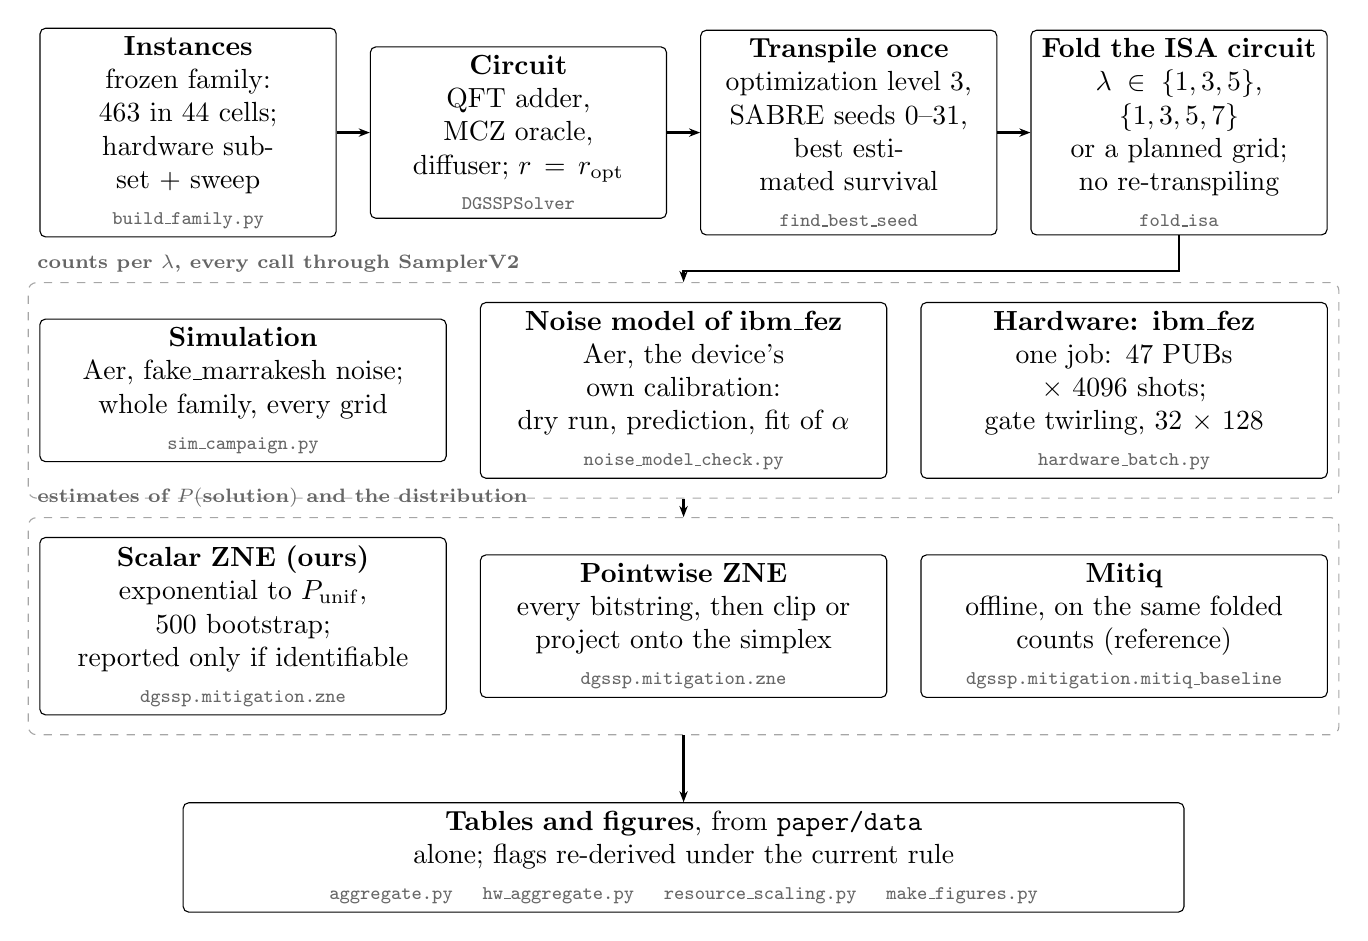
\begin{tikzpicture}[
    node distance=0.45cm and 0.42cm,
    box/.style={draw, rounded corners=2pt, align=center, inner sep=3pt,
                text width=#1, minimum height=1.6cm},
    box/.default=3.55cm,
    run/.style={box=4.95cm, minimum height=1.35cm},
    est/.style={box=4.95cm, minimum height=1.25cm},
    flow/.style={-{Stealth[length=4pt]}, thick},
    group/.style={draw=black!35, dashed, rounded corners=3pt, inner sep=4pt},
    head/.style={font=\scriptsize\bfseries, text=black!60, anchor=south west},
  ]
  % Row 1: one circuit per instance, shared by every executor.
  \node[box] (inst) {\textbf{Instances}\\ frozen family: 463 in 44 cells;\\
    hardware subset + sweep\\[1pt] {\tool build\_family.py}};
  \node[box, right=of inst] (circ) {\textbf{Circuit}\\ QFT adder, MCZ oracle,\\
    diffuser; $r = r_\mathrm{opt}$\\[1pt] {\tool DGSSPSolver}};
  \node[box, right=of circ] (isa) {\textbf{Transpile once}\\ optimization level 3,
    SABRE seeds 0--31,\\ best estimated survival\\[1pt] {\tool find\_best\_seed}};
  \node[box, right=of isa] (fold) {\textbf{Fold the ISA circuit}\\
    $\lambda \in \{1, 3, 5\}$, $\{1,3,5,7\}$\\ or a planned grid; no re-transpiling\\[1pt]
    {\tool fold\_isa}};

  % Row 2: the three executors, all through SamplerV2 (qiskit-ibm-runtime).
  % Centred under the middle of row 1.
  \node[run, anchor=north] (ex2) at ($(circ.south)!0.5!(isa.south) + (0,-0.95)$)
    {\textbf{Noise model of ibm\_fez}\\ Aer, the device's own calibration:\\
    dry run, prediction, fit of $\alpha$\\[1pt] {\tool noise\_model\_check.py}};
  \node[run, left=of ex2] (ex1) {\textbf{Simulation}\\ Aer, fake\_marrakesh noise;\\
    whole family, every grid\\[1pt] {\tool sim\_campaign.py}};
  \node[run, right=of ex2] (ex3) {\textbf{Hardware: ibm\_fez}\\ one job: 47 PUBs
    $\times$ 4096 shots;\\ gate twirling, 32 $\times$ 128\\[1pt] {\tool hardware\_batch.py}};
  \begin{scope}[on background layer]
    \node[group, fit=(ex1)(ex2)(ex3), inner ysep=7pt] (execs) {};
  \end{scope}
  \node[head] at (execs.north west) {counts per $\lambda$, every call through SamplerV2};

  % Row 3: three estimators on the same counts.
  \node[est, below=0.95cm of ex1] (zne) {\textbf{Scalar ZNE (ours)}\\ exponential to
    $P_\mathrm{unif}$, 500 bootstrap;\\ reported only if identifiable\\[1pt]
    {\tool dgssp.mitigation.zne}};
  \node[est, right=of zne] (pw) {\textbf{Pointwise ZNE}\\ every bitstring, then clip
    or\\ project onto the simplex\\[1pt] {\tool dgssp.mitigation.zne}};
  \node[est, right=of pw] (mitiq) {\textbf{Mitiq}\\ offline, on the same folded\\
    counts (reference)\\[1pt] {\tool dgssp.mitigation.mitiq\_baseline}};
  \begin{scope}[on background layer]
    \node[group, fit=(zne)(pw)(mitiq), inner ysep=7pt] (ests) {};
  \end{scope}
  \node[head] at (ests.north west) {estimates of $P(\text{solution})$ and the distribution};

  % Row 4: tables and figures from data/ alone.
  \node[box=12.5cm, minimum height=0.95cm, below=0.85cm of ests.south, anchor=north] (out)
    {\textbf{Tables and figures}, from \texttt{paper/data} alone; flags re-derived under
    the current rule\\[1pt] {\tool aggregate.py \quad hw\_aggregate.py \quad
    resource\_scaling.py \quad make\_figures.py}};

  \draw[flow] (inst) -- (circ);
  \draw[flow] (circ) -- (isa);
  \draw[flow] (isa) -- (fold);
  \draw[flow] (fold.south) |- ++(0,-0.45) -| (execs.north -| ex2.north);
  \draw[flow] (execs.south -| pw.north) ++(0,0) -- (ests.north -| pw.north);
  \draw[flow] (ests.south) -- (out.north);
\end{tikzpicture}
\end{document}
